\subsection{Problem Definition}
\label{sec:motion_planning_model}

% Bài toán hoạch định chuyển động cho robot tự hành đặt ra yêu cầu tìm một quỹ đạo
% kết nối trạng thái khởi đầu với trạng thái đích trong môi trường chứa vật cản,
% đồng thời thỏa mãn các ràng buộc về an toàn hình học và giới hạn động học của hệ.

Motion planning problem for autonomous robots requires finding a trajectory that connects the start state to the goal state in an environment with obstacles, while satisfying geometric safety constraints and the system's dynamic limits.

% Xét quỹ đạo liên tục $\mathbf{x}(t) \colon [0, T] \to \mathbb{R}^d$, trong đó
% $d$ là số chiều của không gian cấu hình và $T > 0$ là thời gian thực hiện.
% Quỹ đạo phải khả vi đến bậc $K$, tức là
% $\frac{\mathrm{d}^k \mathbf{x}}{\mathrm{d}t^k}$ tồn tại và liên tục với $k = 1, \ldots, K$.

Consider a continuous trajectory $\mathbf{x}(t) \colon [0, T] \to \mathbb{R}^d$, where
$d$ is the dimension of the configuration space and $T > 0$ is the execution time.
The trajectory must be differentiable up to order $K$, i.e.,
$\frac{\mathrm{d}^k \mathbf{x}}{\mathrm{d}t^k}$ exists and is continuous for $k = 1, \ldots, K$.

% Hàm mục tiêu tổng quát được định nghĩa là
Objective function is defined as
\begin{equation}
    \psi(\mathbf{x}(\cdot),\, T)
    :=
    a\,\Phi(T)
    + \sum_{m=1}^{M} b_m
      \int_0^T
      \left\| \frac{\mathrm{d}^m \mathbf{x}}{\mathrm{d}t^m}(t) \right\|^2
      \mathrm{d}t,
    \label{eq:cost_general}
\end{equation}

% trong đó $\Phi(T)$ là chi phí liên quan đến thời gian, $m$ là bậc đạo hàm cần
% tối ưu hóa, và $a, b_m > 0$ là các hệ số trọng số.
which $\Phi(T)$ is the time-related cost, $m$ is the order of derivative to be optimized, and $a, b_m > 0$ are weighting coefficients.

% Bài toán hoạch định chuyển động tổng quát được phát biểu như sau:
Motion planning problem can be formulated as follows:
\begin{equation}
\begin{aligned}
    \min_{\mathbf{x}(\cdot),\; T} \quad
    & \psi(\mathbf{x}(\cdot), T) \\
    \mathrm{s.t.} \quad
    & \mathbf{x}(0) = \mathbf{x}_{\mathrm{start}},
      \quad
      \mathbf{x}(T) = \mathbf{x}_{\mathrm{goal}}, \\
    & \mathbf{x}(t) \in \mathcal{C}_{\mathrm{free}},
      \quad \forall\, t \in [0, T], \\
    & \frac{\mathrm{d}^k \mathbf{x}}{\mathrm{d}t^k}(t) \in \mathcal{D}_k,
      \quad k = 1, \ldots, K,\; \forall\, t \in [0, T], \\
    & T_{\min} \leq T \leq T_{\max}.
\end{aligned}
\label{eq:planning_problem}
\end{equation}

% Ràng buộc $\mathbf{x}(t) \in \mathcal{C}_{\mathrm{free}}$ yêu cầu quỹ đạo tránh
% va chạm tại mọi thời điểm; ràng buộc $\frac{\mathrm{d}^k \mathbf{x}}{\mathrm{d}t^k}
% \in \mathcal{D}_k$ giới hạn các đạo hàm bậc $k$ trong tập khả thi $\mathcal{D}_k$,
% phản ánh giới hạn vật lý của hệ như vận tốc tối đa, gia tốc tối đa, và độ trơn (jerk).
% Thách thức trung tâm nằm ở tập $\mathcal{C}_{\mathrm{free}}$: do sự hiện diện của
% vật cản, $\mathcal{C}_{\mathrm{free}}$ là tập phi lồi, khiến bài
% toán~\eqref{eq:planning_problem} trở thành phi lồi và NP-hard trong trường hợp
% tổng quát~\cite{LaValle2006}.

The constraint $\mathbf{x}(t) \in \mathcal{C}_{\mathrm{free}}$ requires the trajectory to avoid collisions at all times; the constraint $\frac{\mathrm{d}^k \mathbf{x}}{\mathrm{d}t^k} \in \mathcal{D}_k$ limits the $k$-th derivatives within the feasible set $\mathcal{D}_k$, reflecting the physical limits of the system such as maximum velocity, maximum acceleration, and jerk. The central challenge lies in the set $\mathcal{C}_{\mathrm{free}}$: due to the presence of obstacles, $\mathcal{C}_{\mathrm{free}}$ is a non-convex set, making the problem~\eqref{eq:planning_problem} non-convex and NP-hard in general~\cite{LaValle2006}.

% \subsection{Tách biệt hình học và phân bổ thời gian}
% \label{subsec:path_coord}

% Khi $T$ là biến quyết định, tích phân trong~\eqref{eq:cost_general} có giới hạn trên
% phụ thuộc vào $T$, tạo ra quan hệ phi tuyến giữa hình dạng quỹ đạo và thời gian.
% Một chiến lược thực tiễn là tham số hóa $\mathbf{x}(t)$ qua tọa độ đường đi
% $s \in [0,1]$ thông qua cặp hàm $q(s)$ (hình dạng hình học) và $h(s)$ (phân bổ thời
% gian), sao cho $\mathbf{x}(t) = q(h^{-1}(t))$~\cite{BobrowDubowskyGibson1985TimeOptimal}.
% Cách tách biệt này giúp áp đặt các ràng buộc về tính mượt mà lên $q(s)$ và $h(s)$
% một cách độc lập; tuy nhiên, các ràng buộc về gia tốc và đạo hàm bậc cao thường mất
% tính lồi trong hệ tọa độ này~\cite{MarcucciEtAl2023MotionPlanning}.

% Hai hướng tiếp cận trong chương này xử lý tính phi lồi của
% bài toán~\eqref{eq:planning_problem} theo hai cách bổ sung cho nhau.
% \textbf{Hướng tiếp cận GCS-Bézier} (Phần~\ref{sec:gcs_approach}) phân hoạch
% $\mathcal{C}_{\mathrm{free}}$ thành các vùng lồi và tham số hóa quỹ đạo bằng đường
% cong Bézier, khai thác tính chất bao lồi để đảm bảo an toàn hình học, hướng đến
% nghiệm tốt nhất và trong đa số trường hợp cận tối ưu toàn cục.
% \textbf{Hướng tiếp cận GCS-DMS} (Phần~\ref{sec:ocp_dms_approach}) mô hình hóa
% trực tiếp phương trình động lực học $\dot{x} = f(x, u)$ và giải bài toán điều khiển
% tối ưu bằng Direct Multiple Shooting kết hợp hàm cản logarit, đảm bảo tính khả thi
% về mặt động lực học tại mọi thời điểm liên tục.


%
\subsection{GCS}
\label{subsec:gcs_framework}

% Đồ thị của các Tập Lồi (Graphs of Convex Sets -- GCS) là một khuôn khổ tối ưu hóa
% hợp nhất giải quyết đồng thời hai thành phần vốn tách biệt trong hoạch định chuyển
% động: chọn đường đi rời rạc trên đồ thị và tối ưu hóa biến hình học liên tục trong
% mỗi vùng~\cite{MarcucciEtAl2023GCS}.
Graph of Convex Sets (GCS) is a unified optimization framework that simultaneously addresses two components that are traditionally treated separately in motion planning: selecting a discrete path on a graph and optimizing continuous geometric variables within each region~\cite{MarcucciEtAl2023GCS}.

% Khác với bài toán đường đi ngắn nhất cổ điển -- nơi chi phí cạnh là hằng số vô hướng
% -- GCS gắn mỗi đỉnh với một biến quyết định liên tục nằm trong một tập lồi, và chi
% phí của mỗi cạnh là hàm lồi của các biến tại hai đỉnh liên thuộc.
% Cấu trúc này cho phép đặt bài toán hoạch định quỹ đạo -- bao gồm đồng thời việc chọn
% chuỗi vùng an toàn và tối ưu hóa hình dạng quỹ đạo -- thành một bài toán tối ưu hóa
% thống nhất, như minh họa trong Hình~\ref{fig:gcs_optimization}.
Different from the classical shortest path problem, where edge costs are scalar constants, GCS associates each vertex with a continuous decision variable within a convex set, and the cost of each edge is a convex function of the variables at its two endpoints. This structure allows the motion planning problem - which involves both selecting a sequence of safe regions and optimizing the trajectory shape—to be formulated as a unified optimization problem, as illustrated in Figure~\ref{fig:gcs_optimization}.

\begin{figure}[htbp]
  \centering
  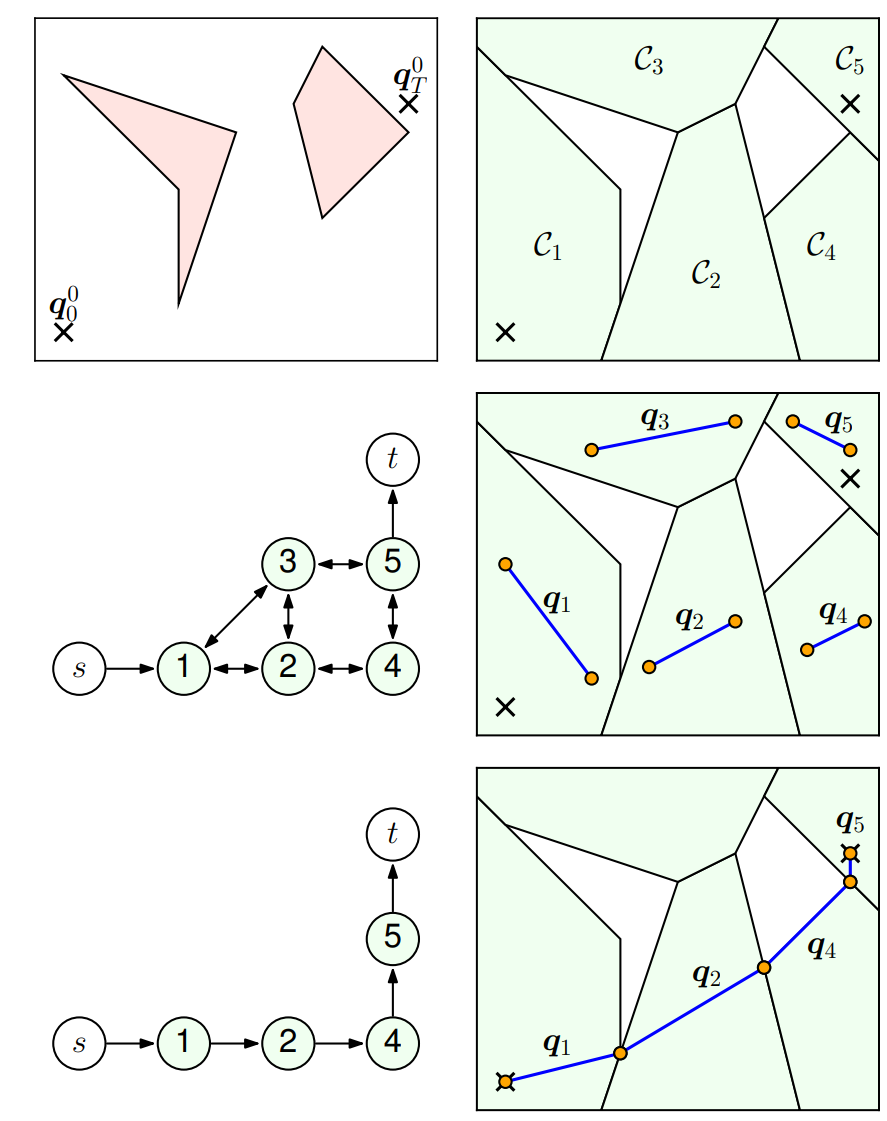
\includegraphics[width=0.85\textwidth]{2-Techical-background/imgs/gcs_spp.png}
  \caption[Minimum-length trajectory planning as an SPP in GCS]{%
    Minimizing the trajectory length can be formulated as a Shortest Path
    Problem (SPP) in GCS~\cite{MarcucciEtAl2023GCS}.
    \emph{Top left}: Environment with two obstacles (pink), the initial
    configuration $q_0^0$ and target configuration $q_T^0$.
    \emph{Top right}: Partition of the free space into convex regions
    $\mathcal{C}_i$.
    \emph{Middle left}: Intersection graph of the partition; the source vertex $s$
    and target vertex $t$ represent boundary points.
    \emph{Middle right}: Local trajectory segments $q_i$ are assigned arbitrarily,
    satisfying the corresponding containment constraints for each convex region.
    \emph{Bottom}: Once the path on the graph is determined, the continuous cost
    functions and constraints jointly enforce the geometry of the entire connected
    trajectory.}
  \label{fig:gcs_optimization}
\end{figure}

\subsubsection{Shortest Path Problem in GCS}
\label{subsubsec:spp_gcs}

A GCS is defined as a directed graph $G = (V, E)$, where each vertex
$v \in V$ is associated with a continuous decision variable $x_v$ lying in a
nonempty compact convex set $\mathcal{X}_v \subset \mathbb{R}^{n_v}$. In the
context of motion planning, $\mathcal{X}_v$ is typically constructed to encode the
parameters of the trajectory segment lying in the corresponding collision-free
convex region of the configuration space. Each edge $e = (u, v) \in E$ specifies
a transition between vertices: every edge imposes an auxiliary convex constraint
$(x_u, x_v) \in \mathcal{X}_e$ and is weighted by a proper closed convex cost
function $\ell_e \colon \mathbb{R}^{n_u + n_v} \to \mathbb{R} \cup \{+\infty\}$.
It is important to note that $\ell_e$ need not be a metric; symmetry and the
triangle inequality are not required~\cite{MarcucciEtAl2023GCS}.

The goal of the SPP in GCS is to determine a path $p$ from the source vertex $s$
to the target vertex $t$ such that the total cost along the path is minimized,
while the continuous variables at each vertex and edge along the path satisfy the
corresponding feasible sets. This problem can be written formally as:
\begin{equation}
  \begin{aligned}
    \min_{p,\; \{x_v\}_{v \in p}} \quad
     & \sum_{(u,v) \in E_p} \ell_{(u,v)}(x_u, x_v)                  \\
    \mathrm{s.t.} \quad
     & p \in \mathcal{P},                                           \\
     & x_v \in \mathcal{X}_v, \quad \forall v \in p,                \\
     & (x_u, x_v) \in \mathcal{X}_e, \quad \forall e=(u,v) \in E_p,
  \end{aligned}
  \label{eq:gcs_spp}
\end{equation}
where $\mathcal{P}$ is the set of all simple paths from $s$ to $t$, and $E_p$ is
the set of edges belonging to path $p$.

By encoding the path selection with binary variables $y_e \in \{0, 1\}$ and applying
the network flow conservation law, problem~\eqref{eq:gcs_spp} can be rewritten
in equivalent form as a Mixed-Integer Nonlinear Program (MINLP):
\begin{subequations}
  \label{eq:gcs_minlp}
  \begin{align}
    \underset{y,\; x}{\mathrm{minimize}} \quad
     & \sum_{e=(u,v) \in E} y_e\, \ell_e(x_u, x_v)
    \label{eq:gcs_obj_milp}                                                  \\
    \mathrm{subject\ to} \quad
     & \sum_{e \in \mathcal{E}^+(u)} y_e - \sum_{e \in \mathcal{E}^-(u)} y_e
    = \delta_u,
    \quad \forall u \in V,
    \label{eq:flow_conservation}                                             \\
     & (x_u, x_v) \in \mathcal{X}_e,
    \quad \forall e=(u,v) \in E,
    \label{eq:edge_constraint}                                               \\
     & x_v \in \mathcal{X}_v,
    \quad \forall v \in V,
    \label{eq:vertex_constraint}                                             \\
     & y_e \in \{0, 1\},
    \quad \forall e \in E.
    \label{eq:binary_variable}
  \end{align}
\end{subequations}
The binary variable $y_e$ indicates whether edge $e$ belongs to the selected path
($y_e = 1$) or not ($y_e = 0$).
The flow conservation constraints~\eqref{eq:flow_conservation} ensure that the
active edges form a valid path from $s$ to $t$, where $\delta_u = 1$ at the
source, $\delta_u = -1$ at the target, and $\delta_u = 0$ at every intermediate
vertex.
Constraints~\eqref{eq:edge_constraint} and~\eqref{eq:vertex_constraint} enforce
that the continuous variables lie in the corresponding feasible set at each
vertex and edge.
The bilinear coupling between $y_e$ and $x_v$ in the objective
function~\eqref{eq:gcs_obj_milp} renders the problem nonconvex; this is the central
challenge addressed by the perspective-relaxation technique introduced later.

\begin{figure}[htbp]
  \centering
  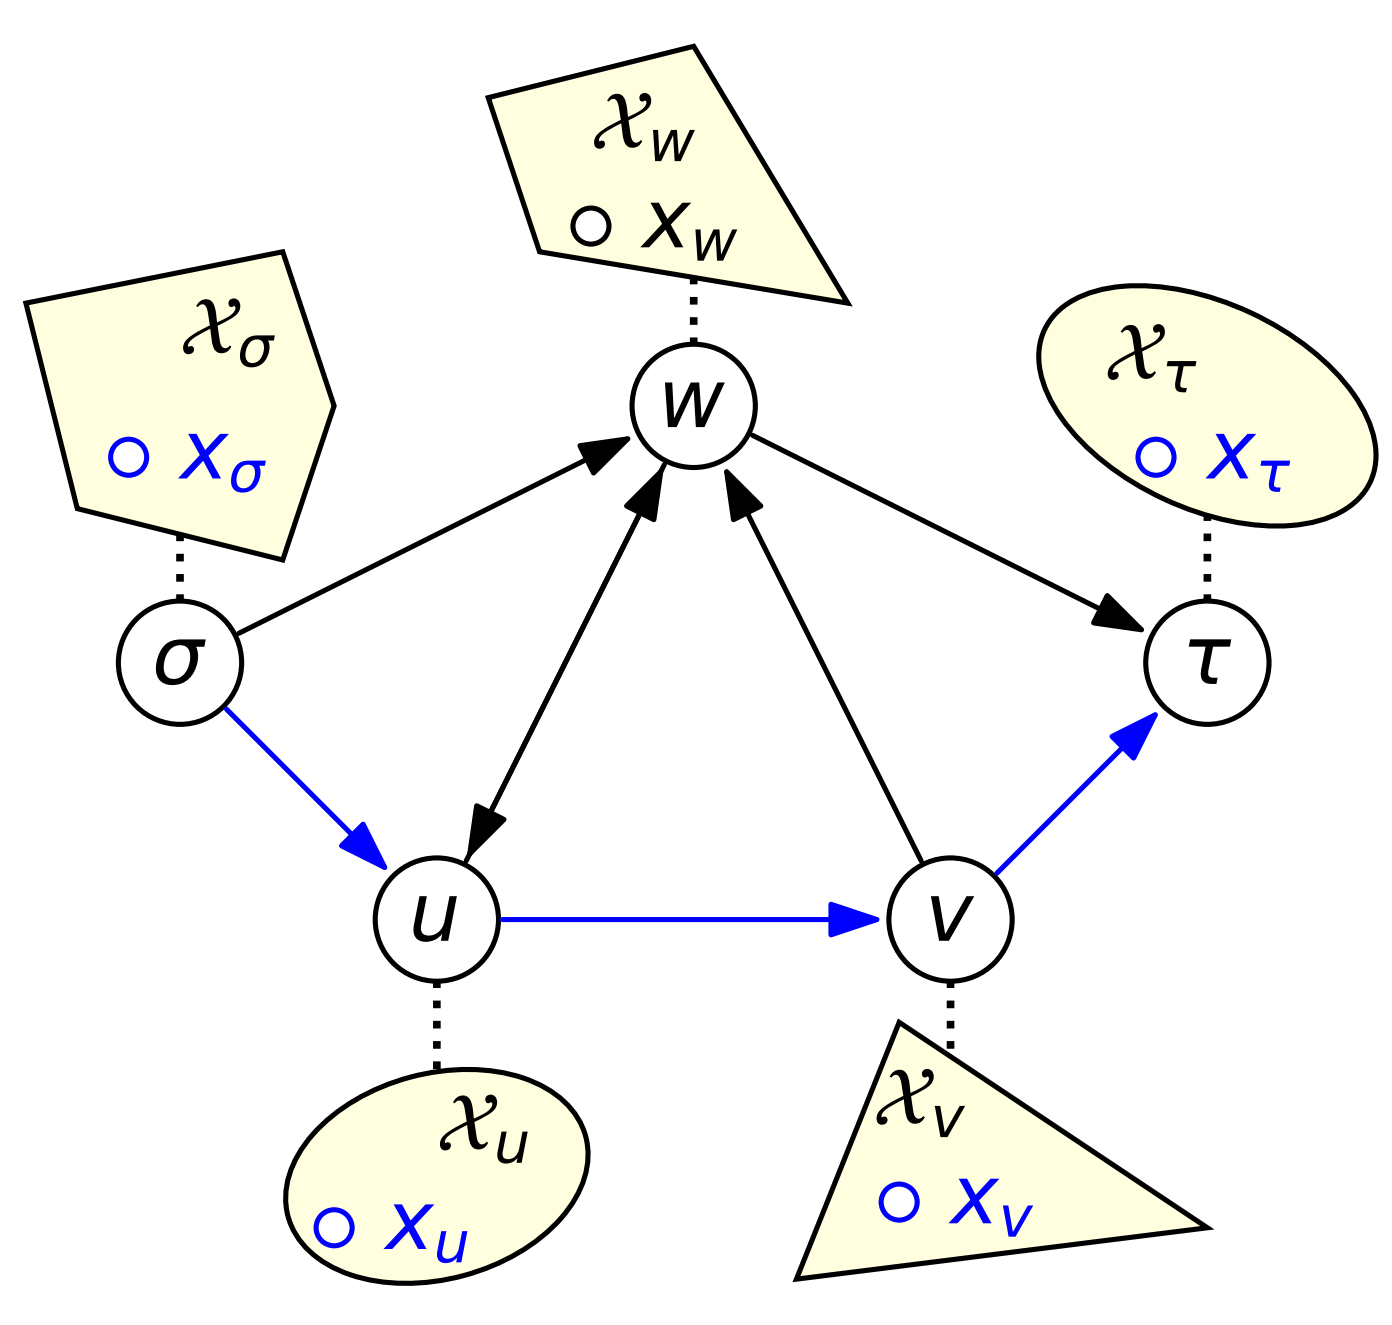
\includegraphics[width=0.5\textwidth]{2-Techical-background/imgs/gcs_set.png}
  \caption[Illustration of the SPP in GCS]{%
    Illustration of the SPP in GCS~\cite{MarcucciEtAl2023GCS}.
    Each vertex $i \in \{\sigma, u, v, w, \tau\}$ is associated with a continuous
    variable $x_i$ in the convex set $\mathcal{X}_i$.
    The weight of each edge is a convex function of the variables at its two
    endpoints.
    The blue path $p = (\sigma, u, v, \tau)$ represents a feasible solution of the
    discrete component; the total cost depends on the optimal values of
    $x_\sigma, x_u, x_v, x_\tau$, but is independent of $x_w$ because vertex $w$
    is not on the path.}
  \label{fig:spp_gcs}
\end{figure}

\subsubsection{Complexity Analysis}
\label{subsubsec:gcs_complexity}

The shortest-path problem in Graphs of Convex Sets (GCS) is fundamentally
different from the classical shortest-path problem on a weighted graph. In the
classical SPP, each edge $e \in E$ is assigned a scalar weight $c_e$, and the
cost of a path is simply the sum of these weights. Therefore, when all edge
weights are nonnegative, the problem can be solved efficiently by Dijkstra's
algorithm or equivalent variants~\cite{AhujaMagnantiOrlin1993}.

In contrast, in GCS each vertex $v$ is associated with a convex set $X_v$ and a
continuous variable $x_v \in X_v$. The cost of edge $e=(u,v)$ is no longer a
predefined constant, but a convex function
\[
  \ell_e(x_u,x_v),
\]
that depends on the continuous variables at both endpoints. Hence, a solution to
the GCS shortest-path problem must simultaneously determine two components: the
discrete path on the graph and the continuous variables associated with the
chosen vertices and edges \cite{MarcucciEtAl2023GCS}. This coupling between
discrete and continuous decisions is precisely why GCS-SPP cannot be treated as a
classical SPP by simply redefining edge weights.

% \begin{proof}[Lập luận độ phức tạp]
%   Giả sử tồn tại một phép biến đổi đa thức đưa mọi thể hiện của SPP trong GCS
%   về một thể hiện SPP cổ điển sao cho nghiệm tối ưu của hai bài toán tương ứng
%   với nhau. Khi đó, nếu thể hiện SPP cổ điển thu được thuộc lớp có thể giải trong
%   thời gian đa thức, chẳng hạn đồ thị không chu trình hoặc đồ thị có trọng số
%   không âm, thì ta sẽ thu được một thuật toán đa thức cho SPP trong GCS.

%   Tuy nhiên, SPP trong GCS đã được chứng minh là NP-hard ngay cả trong các trường
%   hợp mà đồ thị cơ sở là không chu trình và các chi phí là không âm
%   \cite{MarcucciEtAl2023GCS,Marcucci2024Thesis}. Nói cách khác, hai điều kiện vốn
%   làm cho SPP cổ điển trở nên dễ giải không đủ để làm cho SPP trong GCS trở thành
%   bài toán đa thức. Vì vậy, nếu phép quy giảm nói trên tồn tại, ta sẽ suy ra rằng
%   một bài toán NP-hard có thể được giải trong thời gian đa thức. Điều này mâu
%   thuẫn với giả thiết chuẩn $\mathrm{P}\neq\mathrm{NP}$.
% \end{proof}

In the context of this project, the key point is not simply the bilinear nature of
the expression $y_e \ell_e(\cdot)$ in the mixed-integer formulation, but the fact
that the entire GCS structure cannot be replaced by a discrete graph with fixed
edge weights. The reason is that the effective weight of an edge is only defined
after the continuous variables in the adjacent convex regions have been chosen.
Therefore, assigning a single weight to each edge beforehand would discard
geometric information about the trajectory inside the convex regions.

The connection to the Hamiltonian problem helps illustrate the origin of this
hardness. In the classical SPP with nonnegative fixed weights, the objective
``shortest path'' typically favors using fewer edges. In contrast, in GCS, since
continuous variables can be optimized along the path, a convex edge cost can lead
the problem to prefer paths with more vertices. A canonical construction is to set
\[
  X_s=\{0\}, \qquad
  X_t=\{1\}, \qquad
  X_v=[0,1] \quad \forall v\neq s,t,
\]
and use the edge cost
\[
  \ell_{uv}(x_u,x_v)=\|x_v-x_u\|_2^2 .
\]
For a fixed path with $\ell$ edges from $s$ to $t$, the continuous variables can be
spread evenly over the interval $[0,1]$, yielding an optimal total cost of the form
\[
  \frac{1}{\ell}.
\]
Thus, minimizing the cost is equivalent to maximizing the number of edges in the
path. In the extreme case, the optimal solution corresponds to a path passing through
all vertices, which is similar in nature to the Hamiltonian path problem
\cite{Marcucci2024Thesis}. This example shows that GCS-SPP is not merely a
classical SPP with redefined weights; it is a discrete-continuous optimization
problem in which the geometry of the convex sets directly affects the combinatorial
selection.

\subsubsection{Vertex and Edge Model in Motion Planning}
\label{subsubsec:gcs_vertex_edge}

In the motion-planning context, the components of a GCS are specified to reflect
both the geometric structure of the configuration space and the dynamical
constraints.

Each vertex $v \in V$ corresponds to a collision-free convex region $Q_v$ in
configuration space. The decision variable $x_v \in \mathbb{R}^{n_v}$ associated
with $v$ represents the parameters of the local trajectory segment; the dimension
$n_v$ is local to each vertex and depends on the chosen trajectory parameterization.
The variable $x_v$ is constrained to lie in a compact convex set
$\mathcal{X}_v \subset \mathbb{R}^{n_v}$, constructed to ensure that the trajectory
segment stays inside $Q_v$ and satisfies the dynamic limits.

With a Bézier-parameterized trajectory of degree $d$, the variable at vertex $v$
consists of the spatial control points $\mathbf{r}_{v,k} \in \mathbb{R}^{n_c}$ and
the time control points $h_{v,k} \in \mathbb{R}$ ($k = 0, \ldots, d$), where $n_c$
is the dimension of the configuration space. The set $\mathcal{X}_v$ is described
by four groups of constraints:
\begin{align}
   & \mathbf{r}_{v,k} \in Q_v,
  \quad k = 0, \ldots, d,
  \label{eq:geo_containment}                       \\
   & \dot{h}_{v,k} \ge \dot{h}_{\min} > 0,
  \quad k = 0, \ldots, d-1,
  \label{eq:time_scaling}                          \\
   & \dot{\mathbf{r}}_{v,k} \in \dot{h}_{v,k}\, D,
  \quad k = 0, \ldots, d-1,
  \label{eq:dynamic_limits}                        \\
   & h_{v,0} \ge 0,
  \quad h_{v,d} \le T_{\max},
  \label{eq:duration_bounds}
\end{align}
where $\dot{\mathbf{r}}_{v,k} := \mathbf{r}_{v,k+1} - \mathbf{r}_{v,k}$ is the
spatial control-point increment, $\dot{h}_{v,k} := h_{v,k+1} - h_{v,k}$ is the
time control-point increment, and $D \subset \mathbb{R}^{n_c}$ is a convex set of
velocity bounds.
Constraint~\eqref{eq:geo_containment} ensures that each spatial control point lies
inside the safe region $Q_v$; together with the convex-hull property of Bézier
curves, this implies that the curve $\mathbf{q}_v(s)$ remains entirely within $Q_v$
for all continuous times.
Constraint~\eqref{eq:time_scaling} ensures that the time parameterization is
strictly monotone, with $\dot{h}_{\min} = 10^{-6}$ in practice to avoid numerical
degeneracy.
Constraint~\eqref{eq:dynamic_limits} bounds the velocity in a convex form jointly
in $(\dot{\mathbf{r}}_{v,k}, \dot{h}_{v,k})$, while constraint~\eqref{eq:duration_bounds}
imposes the start and end time bounds of each segment.

Each edge $e = (u, v) \in E$ represents a transition between two vertices. The
edge feasibility set $\mathcal{X}_e \subseteq \mathbb{R}^{n_u + n_v}$ imposes
compatibility conditions on $(x_u, x_v)$, including continuity constraints $C^0$,
$C^1$, and higher-order conditions between adjacent trajectory segments. The edge
cost function $\ell_e \colon \mathbb{R}^{n_u + n_v} \to \mathbb{R}$ is convex and
evaluates the transition cost based on both $x_u$ and $x_v$.

\subsubsection{Edge Cost Specification}
\label{subsubsec:gcs_cost}

The choice of the cost function $\ell_e(x_u, x_v)$ determines the physical meaning
of the resulting optimal trajectory. Depending on the objective, two main classes
of costs are used in this project.

\paragraph{Geometric Path-Length Cost}\mbox{}\\

When the objective is to minimize the geometric length of the path through convex
regions, the edge cost is constructed from the Euclidean distance between the
variables at the two vertices. The squared $\ell_2$ norm,
\[
  \ell_e(x_u, x_v) = \|x_v - x_u\|_2^2,
\]
is a natural quadratic function compatible with quadratic programming (QP)
solvers. The standard $\ell_2$ norm,
\[
  \ell_e(x_u, x_v) = \|x_v - x_u\|_2,
\]
can be modeled using second-order cone programming (SOCP) because of the convexity
of the norm and scales linearly with the Euclidean distance, providing an
accurate geometric measure of path length.

\paragraph{Dynamic Trajectory Cost}\mbox{}\\

With Bézier parameterization, the variable $x_v$ includes both spatial control
points and time control points, allowing the construction of a composite objective
with three terms.

The time cost, designed to favor shorter execution time while preserving convexity,
is defined as:
\begin{equation}
  J_t = w_t\, T_v,
  \label{eq:time_cost}
\end{equation}
where $T_v := h_{v,d} - h_{v,0}$ is the execution time of the trajectory segment
at vertex $v$, and $w_t > 0$ is a weighting coefficient.
Since $T_v$ is linear in the decision variables, $J_t$ preserves the convexity of
the objective.

The energy cost, which penalizes the integral of the squared velocity over the
actual time horizon, is defined as:
\begin{equation}
  J_e = \int_0^{T_v} \|\dot{\mathbf{r}}(t)\|_2^2\, \mathrm{d}t.
  \label{eq:energy_cost}
\end{equation}
When expressed through Bézier parameters, $J_e$ becomes a quadratic-over-linear
function of $(\mathbf{r}_{v,k}, T_v)$.
Because the perspective of a convex function preserves convexity, $J_e$ remains
convex in the spatial control points and time variables, enabling joint optimization
of geometry and time allocation in the same MICP problem.

To ensure high-order smoothness, such as minimizing jerk, the cost function adds a
regularization term based on higher-order derivatives:
\begin{equation}
  J_s = \sum_{k=0}^{d-2} \|\ddot{\mathbf{r}}_{v,k}\|_2^2,
  \label{eq:smooth_cost}
\end{equation}
where $\ddot{\mathbf{r}}_{v,k} := \dot{\mathbf{r}}_{v,k+1} - \dot{\mathbf{r}}_{v,k}$
is the second-order difference of the spatial control points.
Unlike $J_e$, the term $J_s$ is a standard quadratic expression in the control
points and does not require a perspective transformation, so it is directly
compatible with QP or SOCP solvers.

% 

%
\subsection{Motion Planning with Bézier Curves}

% 
